%%% Chapter 5 — Base Paper And Its Limitation %%%

\section{Base Paper Analysis}

The proposed framework draws upon and extends the work of Priyadarsini \textit{et al.}~\cite{priyadarsini2025}, titled \textit{AI-Driven Audit Framework for Distributed Multi-Agent Smart Grids}, published in ACM Transactions on Cyber-Physical Systems, 2025. The base paper presents an approach that links anomaly detection with audit optimisation in multi-agent smart grid environments. The main contributions and limitations of this work are discussed below.

\par \vspace{0.35cm}

\noindent
\textbf{Core Approach.}
The base paper proposes a single-layer deviation scoring mechanism for anomaly detection across distributed grid agents. Each agent $i$ at time step $t$ is assigned a deviation score computed as:

\begin{equation}
S_i(t) = w_i \left( d_x + d_y \right)
\label{eq:base_deviation}
\end{equation}

\noindent
where $d_x$ and $d_y$ represent the deviations of the agent's observed measurements from the expected reference profile, and $w_i$ is the weight assigned to the agent based on its criticality. Agents whose scores exceed a predefined threshold are flagged for audit. The audit scheduling component employs Q-learning to determine the allocation of audit resources across the grid, using cost efficiency as the primary reward signal.

\par \vspace{0.35cm}

\noindent
\textbf{Reported Performance.}
The base paper reports the following results on its evaluation configuration:

\begin{table}[H]
\centering
\caption{Performance metrics reported by the base paper~\cite{priyadarsini2025}.}
\label{tab:base_paper_metrics}
\begin{tabular}{|l|c|}
\hline
\textbf{Metric} & \textbf{Value} \\ \hline
Cost Efficiency & 42.5\% \\ \hline
Audit Coverage & 93.8\% \\ \hline
Detection Accuracy & 98.4\% \\ \hline
Risk Mitigation & 87.9\% \\ \hline
\end{tabular}
\end{table}

\noindent
\textbf{Strengths.}
The principal strength of the base paper lies in its explicit coupling of anomaly detection outcomes with audit resource allocation. By linking deviation-based scoring to audit scheduling, the system avoids treating detection and auditing as independent processes and instead enables detection-informed audit prioritisation. The use of reinforcement learning for scheduling introduces adaptability to changing operational conditions.

\par \vspace{0.35cm}

\noindent
\textbf{Limitations.}
Despite these contributions, the base paper has several clear limitations that restrict its applicability to realistic smart grid environments:

\begin{enumerate}
    \item \textbf{Single Detection Modality.} The system relies exclusively on deviation scoring, which captures only instantaneous statistical divergence from expected values. There is no temporal modelling (such as LSTM-based sequence analysis) to detect time-correlated anomalies or gradual drift patterns. This limits the system's ability to identify sophisticated attack types that unfold over multiple time steps.

    \item \textbf{No Live SCADA Integration.} The base paper operates entirely on simulated or offline data. There is no integration with a supervisory control and data acquisition (SCADA) system for live telemetry ingestion, which is a fundamental requirement for operational deployment in real grid environments.

    \item \textbf{No Multi-Layer Detection for Specific Attack Types.} The single-layer deviation approach does not provide specialised detection mechanisms for distinct cyber-physical attack categories such as false data injection (FDI), denial of service (DoS), or man-in-the-middle (MITM) attacks. Each of these attack types exhibits distinct patterns that benefit from dedicated detection logic.

    \item \textbf{No Explicit Experiment/Live Separation.} The base paper does not distinguish between experimental evaluation and live operational monitoring. In a practical deployment, it is essential to maintain separate workspaces to prevent experimental artefacts from contaminating operational decision-making.

    \item \textbf{Limited Operator-Facing Visualisation.} The base paper does not provide a full operational dashboard for real-time monitoring, audit trail inspection, or system health assessment. Operator-facing interfaces are needed for practical adoption in utility environments.

    \item \textbf{No Explainability.} The system does not incorporate any explainability mechanism. Operators receive anomaly flags without per-feature attribution or reasoning, which limits trust and hampers the ability to perform root-cause investigation.

    \item \textbf{Q-Learning Only Scheduling.} The audit scheduling component relies solely on Q-learning. While effective for discrete action selection, Q-learning alone does not support continuous gradient-based optimisation of budget allocation across agents, which can improve cost efficiency in larger deployments.

    \item \textbf{Simple Q-Table State Representation.} The base paper uses a minimal state representation for the Q-table. There is no explicit encoding of the agent's LSTM-derived anomaly probability, its behavioural cluster identity, or the current audit capacity utilisation. This limits the scheduler's ability to differentiate between agents that share a similar raw risk score but differ in their temporal anomaly trajectory or in their operational load context.

    \item \textbf{No Class Imbalance Handling.} The base paper does not describe how training data class imbalance is handled. In smart grid monitoring, normal operation vastly outnumbers anomalous events. Without an explicit mechanism to address this, a standard training objective will be dominated by the majority class, leading to a model that is biased toward predicting normal operation.

    \item \textbf{No Real Benchmark Dataset for LSTM Initialisation.} The base paper does not draw on any publicly available dataset to initialise or validate the LSTM temporal model. Starting from random weights requires significantly more synthetic training data to reach stable performance, and it means the model has no prior knowledge of the physical dynamics or network intrusion patterns that characterise the problem domain.
\end{enumerate}


\section{Extension in Proposed System}

The proposed system addresses each of the identified limitations through the following extensions:

\begin{enumerate}
    \item \textbf{Multi-Layer Detection Pipeline.} The detection architecture is extended from a single deviation layer to a multi-layer pipeline comprising: (a) statistical deviation scoring, (b) LSTM-based temporal anomaly detection, (c) weighted ensemble fusion, and (d) a multi-detector module with four Layer~C sub-detectors: CUSUM-based FDI detection with a shape gate, weighted-rule DoS detection, integrity-and-jump MITM detection, and signature-template physical fault detection, combined by an OR-with-precedence rule and a cross-layer corroboration gate.

    \item \textbf{Weighted Ensemble Fusion.} The deviation score and LSTM anomaly probability are combined through a weighted ensemble with empirically tuned coefficients (deviation weight 0.48, LSTM probability weight 0.52), producing a composite risk score that balances instantaneous and temporal signals.

    \item \textbf{Hybrid Audit Scheduling.} The scheduling component is extended from Q-learning alone to a hybrid approach combining Q-learning for discrete escalation decisions with gradient descent for continuous budget-constrained cost optimisation.

    \item \textbf{Live Rapid SCADA Integration.} The system integrates Rapid SCADA as the supervisory telemetry layer for a 100-agent grid. A PowerShell-based bridge acquires telemetry through the Rapid SCADA Web API and forwards it to the FastAPI backend for real-time processing.

    \item \textbf{Dual Workspace Separation.} The system implements two distinct operational workspaces: \textit{Experiment Running} for simulation, benchmarking, and comparative evaluation; and \textit{Rapid SCADA Live} for operational monitoring and decision support. This separation ensures that experimental configurations do not interfere with live operational data.

    \item \textbf{XAI Explainability with Per-Feature Ranking.} An explainability module generates per-agent, per-feature importance rankings for each anomaly assessment, letting operators see which measurement dimensions contributed most to a given risk score.

    \item \textbf{Five-Method Comparative Validation.} The proposed multi-layer approach is validated against four alternative methods (deviation-only, LSTM-only, Isolation Forest, and One-Class SVM) using identical data and evaluation protocols, for a fair comparison across methods.

    \item \textbf{Full Operational Dashboard.} A Next.js dashboard shows real-time views of agent monitoring, audit trails, risk analytics, threat events, decision explainability, system health, asset topology, and incident timelines.

    \item \textbf{Dual-Dataset LSTM Pre-Training.} To address the absence of benchmark dataset integration in the base paper, the proposed system pre-trains the physical LSTM branch on the UCI Electrical Grid Stability Dataset (10,000 samples, 12 features) and the cyber LSTM branch on the UNSW-NB15 Network Intrusion Dataset. Four composite features are engineered from UNSW-NB15 that map directly onto the simulation's cyber feature space (latency, packet loss, integrity, communication frequency). Pre-training gives each branch prior knowledge of physical instability patterns and network intrusion signatures before the model sees any synthetic grid data.

    \item \textbf{Class Imbalance Handling in LSTM Training.} Focal Loss ($\gamma = 2.0$, $\alpha = 0.65$) replaces standard binary cross-entropy to focus gradient signal on hard minority-class attack samples. A WeightedRandomSampler (positive-class scale 1.40, oversampling scale 1.35) ensures attack events appear frequently within each training mini-batch. Post-training temperature calibration via grid search over $T \in [0.80, 2.20]$ ensures that output probabilities are well-calibrated for downstream ensemble fusion.

    \item \textbf{Extended Q-Table State Space.} The Q-table state is extended from a minimal scalar representation to a four-dimensional tuple: (risk bucket, LSTM probability bucket, K-Means behavioural cluster, audit capacity bucket), producing up to 300 reachable states. An experience replay buffer (capacity 2,000, batch size 32) stabilises Q-value learning. Three risk-sensitive reward modes are supported: expected return, exponential utility ($\beta = -0.05$), and Conditional Value-at-Risk ($\alpha = 10\%$).

    \item \textbf{Temporal Signature Classification and Five-Class Attack Typing.} A temporal pattern classifier identifies the shape of each anomaly trajectory (STEP, RAMP, OSCILLATORY, STABLE) and feeds it into a five-class attack typer that assigns each flagged agent one of: FDI, DoS, MITM, Physical Fault, or Coordinated Chain Attack. This extends attack coverage beyond the three categories considered by the base paper and gives operators a more specific characterisation of each event.
\end{enumerate}


\section{Comparative Summary}

Table~\ref{tab:base_vs_proposed} presents a side-by-side comparison between the base paper and the proposed system across all principal dimensions.

\begin{table}[H]
\centering
\caption{Comparative summary: base paper vs.\ proposed system (N=100).}
\label{tab:base_vs_proposed}
\begin{tabular}{|l|p{3.5cm}|p{5.5cm}|}
\hline
\textbf{Metric / Feature} & \textbf{Base Paper} & \textbf{Proposed System (N=100)} \\ \hline
Detection Accuracy & 98.4\% & 93.85\% \\ \hline
False Positive Rate & 3.2\% & 6.18\% \\ \hline
Recall & 100\% & 98.24\% \\ \hline
Risk Mitigation & 87.9\% & 93.66\% \\ \hline
Cost Efficiency & 42.5\% & 57.28\% \\ \hline
Audit Coverage & 93.8\% & 100\% \\ \hline
Detection Layers & 1 (deviation only) & multi-layer (deviation + LSTM + C-1 to C-4) \\ \hline
Attack Types Covered & FDI, DoS, MITM (qualitative) & FDI, DoS, MITM, Physical Fault, Chain Attack (5-class typed) \\ \hline
Q-Table State Space & Minimal scalar representation & 4D tuple: risk $\times$ probability $\times$ cluster $\times$ capacity = 300 states \\ \hline
RL Enhancements & Standard Q-learning & Experience replay, CVaR and exponential utility reward modes \\ \hline
LSTM Pre-Training Data & None & UCI Grid Stability (physical branch), UNSW-NB15 (cyber branch) \\ \hline
Class Imbalance Handling & Not described & Focal Loss ($\gamma=2.0$, $\alpha=0.65$) + WeightedRandomSampler \\ \hline
Scheduling & Q-learning only & Hybrid Q-learning + gradient cost optimisation \\ \hline
SCADA Integration & None & Rapid SCADA, 100 agents \\ \hline
Explainability & None & Per-feature XAI with ranked contribution scores \\ \hline
\end{tabular}
\end{table}

\begin{figure}[H]
\centering
\fbox{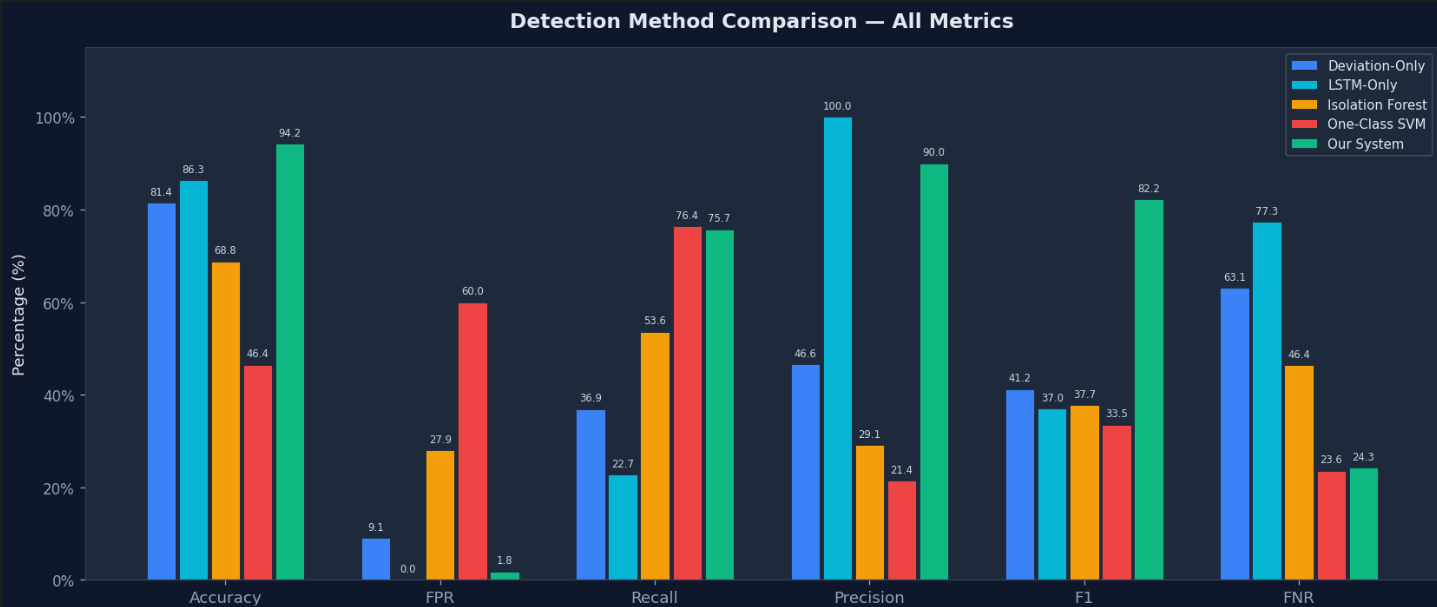
\includegraphics[width=0.95\textwidth]{FigAllMetrciComparison.png}}
\caption{Comparative visualisation of primary performance metrics: base paper vs.\ proposed system.}
\label{fig:all_metric_comparison}
\end{figure}

\par \vspace{0.35cm}
\noindent
\textbf{Reproducibility.} The comparative evaluation was conducted using two Jupyter notebooks included in the project repository: \texttt{basepaper.ipynb} (replication of the base paper's deviation-only scoring on identical synthetic data) and \texttt{method\_comparison\_study.ipynb} (five-method comparative validation). Both notebooks operate on the same synthetic dataset generated by \texttt{grid\_env.py}, so that all methods are evaluated under identical conditions.

\begin{figure}[H]
\centering
\fbox{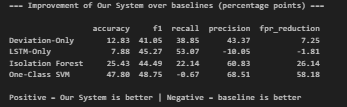
\includegraphics[width=0.95\textwidth]{FigImprovement.png}}
\caption{Improvement deltas across primary metrics relative to the base paper.}
\label{fig:improvement_deltas}
\end{figure}

\noindent
As illustrated in Table~\ref{tab:base_vs_proposed} and Figures~\ref{fig:all_metric_comparison}--\ref{fig:improvement_deltas}, the proposed system improves on the base paper in risk mitigation (93.66\% compared to 87.9\%), cost efficiency (57.28\% compared to 42.5\%), and audit coverage (100\% compared to 93.8\%), and reaches a recall of 98.24\% that the base paper does not report. The detection accuracy of 93.85\% is below the base paper's 98.4\% and the system level false positive rate of 6.18\% is above the base paper's 3.2\%, because the proposed pipeline is tuned for high recall so that very few genuine attacks are missed. Beyond these numbers, the proposed system introduces qualitative capabilities absent from the base paper, including multi-layer detection with per attack typing, SCADA integration, dual workspace separation, and explainability.


\section{Timeline and Development Progress}

Table~\ref{tab:timeline} summarises the four-phase development timeline adopted for this project.

\begin{table}[H]
\centering
\caption{Project development timeline.}
\label{tab:timeline}
\begin{tabular}{|c|l|l|}
\hline
\textbf{Phase} & \textbf{Period} & \textbf{Activities} \\ \hline
1 & July--September 2025 & \begin{tabular}[t]{@{}l@{}}Problem formulation, dataset preparation,\\baseline experimentation\end{tabular} \\ \hline
2 & September 2025--January 2026 & \begin{tabular}[t]{@{}l@{}}Feature engineering, prototype development,\\initial anomaly detection implementation\end{tabular} \\ \hline
3 & January--April 2026 & \begin{tabular}[t]{@{}l@{}}Model refinement, system integration,\\full evaluation across configurations\end{tabular} \\ \hline
4 & April--June 2026 & \begin{tabular}[t]{@{}l@{}}Documentation, system packaging,\\preparation for final presentation and defense\end{tabular} \\ \hline
\end{tabular}
\end{table}

\noindent
The phases overlap because the development was iterative, findings from later phases fed back into earlier design decisions and led to ongoing changes throughout the project.
